\section{Construção de um exemplo}

Introdução à construção do exemplo.

\subsection{O estudo original}

O estudo original buscava avaliar o impacto de intervenções de psicologia positiva conduzidas via internet sobre a percepção de felicidade e
sintomas depressivos \cite{Woodworth2017}, uma tentativa de replicar os resultados obtidos em um trabalho anterior conduzido por Seligman e
colaboradores \cite{Seligman2005}.

\subsubsection{Participantes}

Os participantes foram recrutados por meio de anúncios em veículos de comunicação australianos: páginas web, jornais e uma estação de rádio
local. Um total de 295 participantes completou a fase inicial de pré-teste. O grupo era composto majoritariamente por mulheres ($85,06\%$),
com idades entre 18 e 83 anos ($M=43,76; SD=12,43$); a maior parte dos participantes possuia nível de educação superior ($74,88\%$) e classificou
a própria renda como média ou acima da média ($76\%$) \cite{Woodworth2017, Collins2023}.

\subsubsection{Intervenções}

Os participantes foram distribuídos aleatoriamente em quatro grupos, três grupos experimentais e um grupo de controle; cada um dos três grupos
experimentais recebeu uma intervenção distinta. O primeiro grupo experimental recebeu a intervenção de \emph{visita da gratidão}: os participantes
foram instruídos escrever e entregar uma carta de agradecimento para alguém que lhes tivesse sido gentil no passado. O segundo grupo experimental
recebeu a intervenção de \emph{três coisas boas}: os participantes deveriam anotar três coisas boas que haviam acontecido durante seu dia, justificando
suas escolhas de eventos. O último grupo experimental recebeu a intervenção de \emph{pontos fortes}: os participantes receberam uma intevenção
psicoeducativa sobre forças de caráter e foram aconselhados a buscar maneiras criativas para utilizar suas próprias forças de caráter no cotidiano.
Todas as intervenções tiveram duração de uma semana \cite{Woodworth2017}.

\subsubsection{Controle}

O grupo de controle foi exposto à atividade placebo de \emph{memórias de infância}: os participantes receberam a instrução de reservar um momento ao
final do dia para escrever sobre suas memórias de infância durante uma semana \cite{Woodworth2017}.

\subsubsection{Desfechos}

O estudo avaliou percepção de felicidade por meio do AHI (Authentic Happiness Inventory), um instrumento de autorrelato composto por 24 items. Os itens
são pontuados em uma escala de que vai de 1 a 5 e a pontuação total é calculada pela soma das pontuações obtidas para cada item. Resultados maiores representam
maiores níveis de felicidade \cite{Park2010}.

Sintomas depressivos foram mensurados com a escala CES-D (Center for epidemiologic studies depression scale), um instrumento de autorrelato composto por 20
itens que avaliam a frequência de sintomas em uma escala Likert de 4 pontos. A CES-D é divida em quatro subescalas: afeto deprimido, afeto positivo, queixas
somáticas e problemas interpessoais. A pontuação em uma subescala é calculada pela soma das pontuações obtidas para cada item associado à subescala. A pontuação
total é calculada pela soma das pontuações obtidas para cada subescala. Resultados maiores representam maior severidade dos sintomas depressivos \cite{Radloff1977}.

\subsection{Árvores de decisão}

Árvores de decisão representam uma classe de modelos de aprendizagem de máquina que pode ser usada para tarefas de classificação e regressão, ou seja, são
capazes de fazer predições para valores de variáveis categóricas e numéricas. Elas utilizam uma série de regras de decisão para predizer o desfecho de interesse;
essas regras consistem em verificações feitas sobre os valores de variáveis presentes no conjunto de dados usados no treinamento do modelo \cite{Theobald2021, Bi2019}.

\begin{figure}[h!]
    \centering
    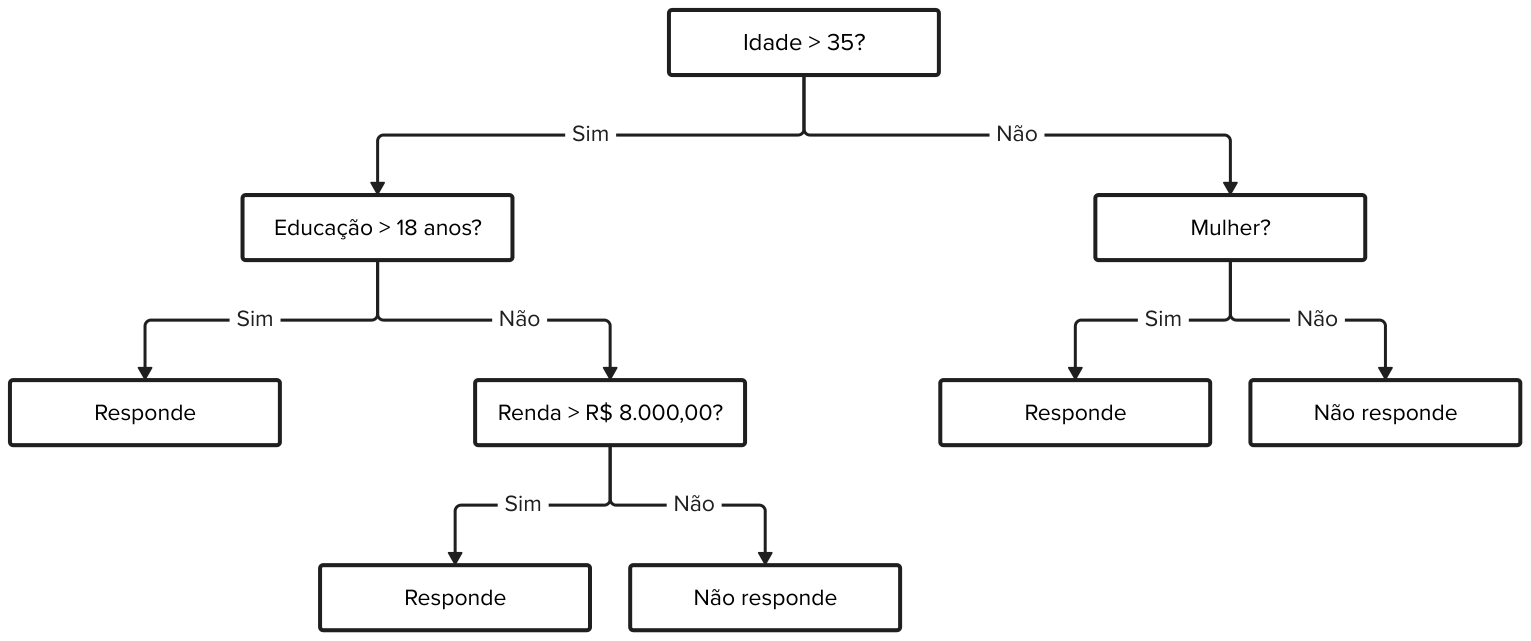
\includegraphics[width=\textwidth]{./03-exemplo/imagens/arvore-exemplo.png}
    \caption{Um exemplo de árvore de decisão construída manualmente.}
    \label{fig:arvore-exemplo}
\end{figure}

Na figura \ref{fig:arvore-exemplo}, temos uma árvore de decisão construída manualmente que realiza a tarefa de predição da resposta a uma intervenção psicoterápica hipotética.
Com acesso às informações necessárias, é possível navegar pela estrutura da árvore e predizer o desfecho que a inteverção teria para uma nova paciente. Para isso, aplicam-se
as regras de decisão sucessivamente a partir do nó inicial, chamado raiz, até alcançar um nó terminal, chamado folha, que contém a informação de desfecho.  Por exemplo,
uma paciente de 38 anos, que estudou durante 15 anos de sua vida e tem uma renda mensal de R\$ $10.000,00$ teria uma previsão de desfecho com resposta positiva à intervenção.

Algoritmos de aprendizagem de máquina para construção de árvores de decisão operam por meio de um processo iterativo: o processamento do conjunto de dados de treinamento
acontece em ciclos que se repetem um determinado número de vezes. Partindo do conjunto de dados de treinamento completo, geram-se as regras de decisão possíveis e seleciona-se
aquela que produz partições mais homogêneas dos dados em relação ao desfecho de interesse. As particões geradas servem como base para o próximo ciclo de processamento. O processo
segue até que se alcance um critério de parada pré-estabelecido, como o tamanho da árvore ou um número mínimo de observações em nós terminais \cite{Bi2019}.

O uso de árvores de decisão apresenta uma série de benefícios. Árvores de decisão exigem um volume de dados menor para realização do treinamento quando comparadas a outras classes
de modelos como as redes neurais artificiais \cite{Theobald2021}. Elas são capazes de modelar relações não lineares entre as variáveis do conjunto de dados, desempenhando melhor
que modelos de regressão linear em contextos onde esse tipo de interação existe \cite{Bi2019}. Além disso, árvore de decisão são facilmente interpretáveis; elas possuem uma representação
gráfica que pode ser compreendida de maneira intutiva, facilitando sua inspeção e a obtenção de insights sobre o processo de tomada de decisão empregado pelo modelo \cite{Bi2019}.
As limitações de modelos de árvore de decisão incluem sua sensibilidade a pequenas perturbações no conjunto de dados, como outliers, e uma inclinação ao sobreajuste: uma adaptação
excessiva às nuances do conjunto de dados de treinamento que prejudica a capacidade de generalização das predições feitas pelo modelo \cite{Bi2019}.

\subsection{Plano de análise de dados}

A.

\subsection{Resultados e discussão}

A.
